%===============================================================================
% Autoři: Michal Bidlo, Bohuslav Křena, Jaroslav Dytrych, Petr Veigend a Adam Herout 2018
\chapter{Úvod}
%Aproximácie, ktoré ako inžinieri používame, nám často zjednodušujú prácu, no zároveň nám pília konár
%pod nohami v prípadoch, keď vyžadujeme neomylnosť a presnosť.
%Obdobná situácia sa vyskytuje aj v optike. Aberácie predstavujú odchýlky, ktoré vznikajú zjedošením
%modelu optických systémov. Ich nesprávne pochope, či dokonca ignorácia, môže viesť k fatálnym chybám
%ako napríklad v prípade Hubblového vesmírneho teleskopu.

\section{Aberácie}
Podľa literatúry je aberácia definovaná ako \textit{odchíľka od idealizovaného modelu Gaussovej
optiky}\cite{hechtoptics}, či \textit{neschopnosť optického systému zaostriť ľúče do jedného bodu}[Wikipédia].

V praxi sú aberácie kolekcia javov, ktoré nastávajú v optických systémoch, a ktorých prítomnosť
obvykle nie je žiadúca. Nakoľko táto práca vznikla na pôde fakulty informačných technológii, budú
nás v tom texte zaujímať negatívne javy, ktoré vznikajú v obraze pri výskyte týchto aberácii.

Aberácie prestavujú odchýlky od ideálneho optického modelu, ktoré sa v ňom nevyskytujú z dôvodu
zjednodušenia formalizov oproti reálnym optickým systémom. Príkladom je \textit{Snellov zákon},
ktorého zjednodušená forma popisuje lom svetla len pre tzv. paraxiálne uhly. \cite{hechtoptics}.

Dôsledkom aberácii sú \textit{optické vady}, ktoré sa prejavujú rozmazaním alebo deformáciou obrazu. V praxi sa tieto
vady riešia rozšírením optickej sústavy o ďalšie prvky, ktoré korigujú ľúče, prípadne pomocou
špecializovaného software-u \cite{automaticRemovalCA}. Softwareové riešenie ale nemusí byť vždy žiaduce nakoľko nemusí
byť fyzikálne presné a môže sa jednať o istú aproximáciu.

Počiatok skúmania aberácii siaha ku matematikovi \textbf{Ludwigovi von Seidelovi} (1821-1896), ktorý
pôsobil na bavorských univerzitách a ktorého jednou z oblastí záujmu bola astronómia. \cite{seidel}
Podstatným krokom pána Seidela bolo zadefinovanie piatich koeficientov v rovnici, ktorá definuje
prechod paprskov šošovkou z pohľadu optiky vyššieho rádu. Vhodnou voľbou týchto koeficientov je 
možné získať predpis hlavných geometrických aberácii. Táto rovnica bola pomenovaná podľa neho a 
v literatúre je označovaná ako \textit{Seidler sums}.

K skúmaniu aberácii ešte skorej prispel aj \textbf{Isaac Newton}, ktorý sa venoval ľudskému vnímaniu svetla a
popísal jav \textit{disperzie svetla} na hranole, ktorá sa týka \textit{chromatickej aberácie}. \cite{elert}

\section{Monochromatické aberácia}
Monochromatické aberácie predstavujú odchýlky, ktoré sa vyskytujú už pri jednej vlnovej dĺžke.
\subsection{Sférická aberacia}
Sférická aberácia nastáva pri dopade rovnobežných ľúčov na sférický rozhranie prostredí. 
Podľa ideálneho modelu šošovky by sa pri dopade na rozhranie zakrivenej šošovky mal ľúč lámať do ohniska šošovky, ktoré
je dané polomerom krivosti danej šošovky. 

Pri dopade sa smer lomu riadi rozšírených Schnellovým zákonom, ktorý je rozšírený o odchýľkový člen, závislý na
uhle. Odchýlka uhlu pri lome spôsobuje, že ľúče nedopadajú do jedného ohniska šošovky, ale sú
rozptýlené v jeho okolí. Táto situácia
je zobrazená na obrázku \ref{saill}.

\begin{figure}[h]
\centering
\label{saill}
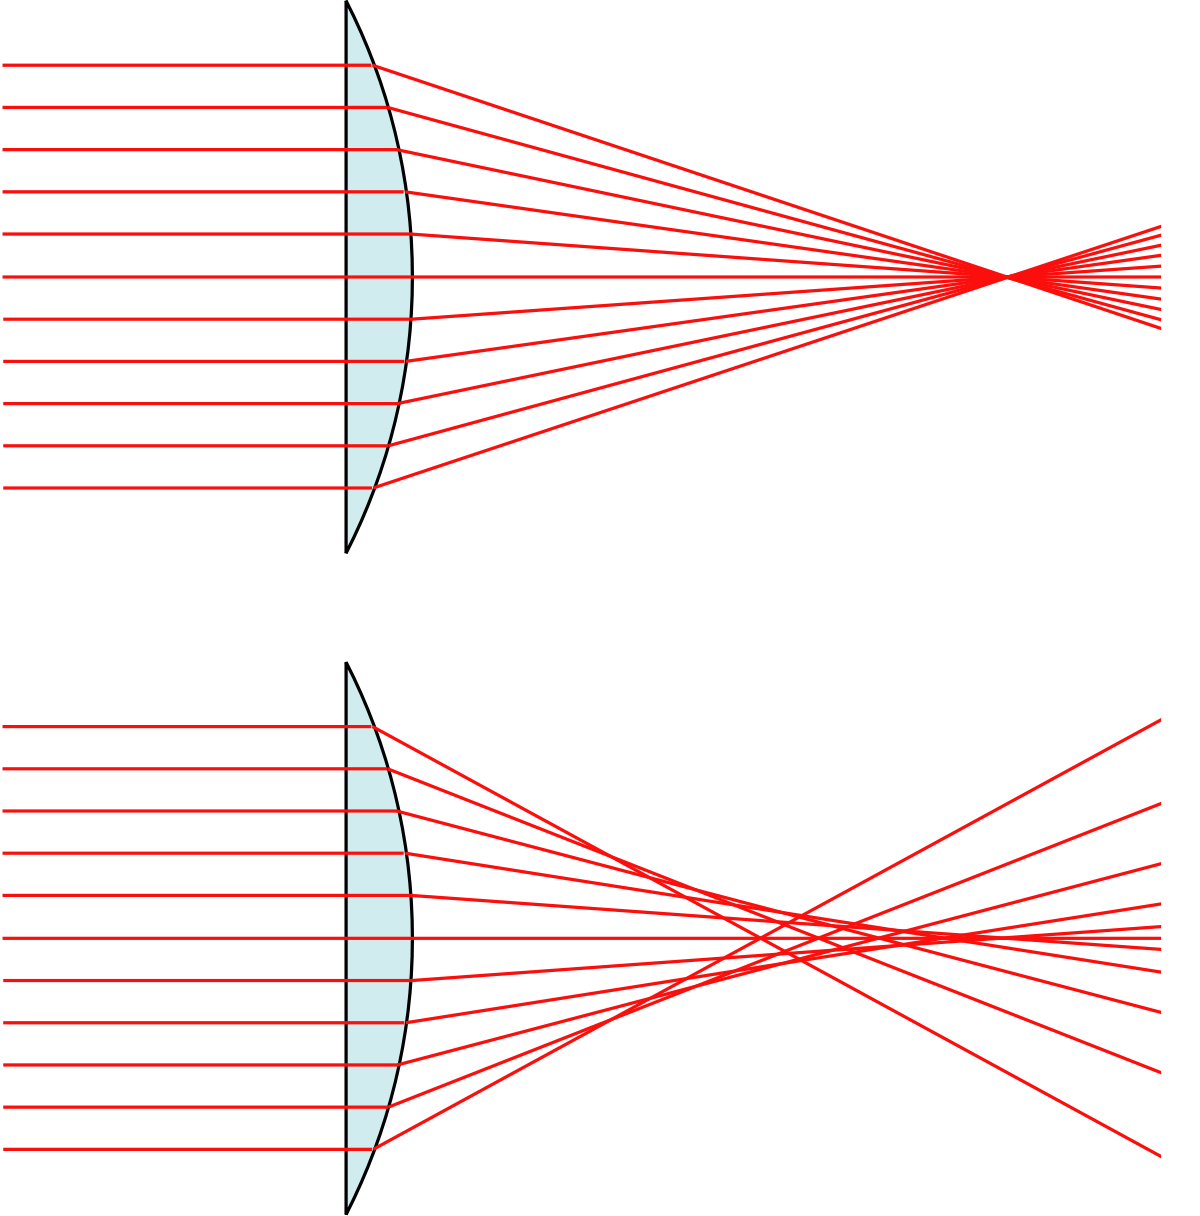
\includegraphics[width=6cm]{obrazky-figures/sphericalAberrationWikipedia.png}
\caption{Ilustrácia sférickej odchíľky. Vplyvom odchíľkového člena sa ľúče na rozhraní nelámu smerom
    do jedného ohniska. Prevzaté z }
\end{figure}

Dôsledkom tohoto javu je rozostretie obrazu pri okrajoch obrazu.  
Riešenie pomocou odlišného tvaru šošovky (apheric lens), ktoré sú ale drahé. https://en.wikipedia.org/wiki/Aspheric\_lens

\begin{figure}[h]
\centering
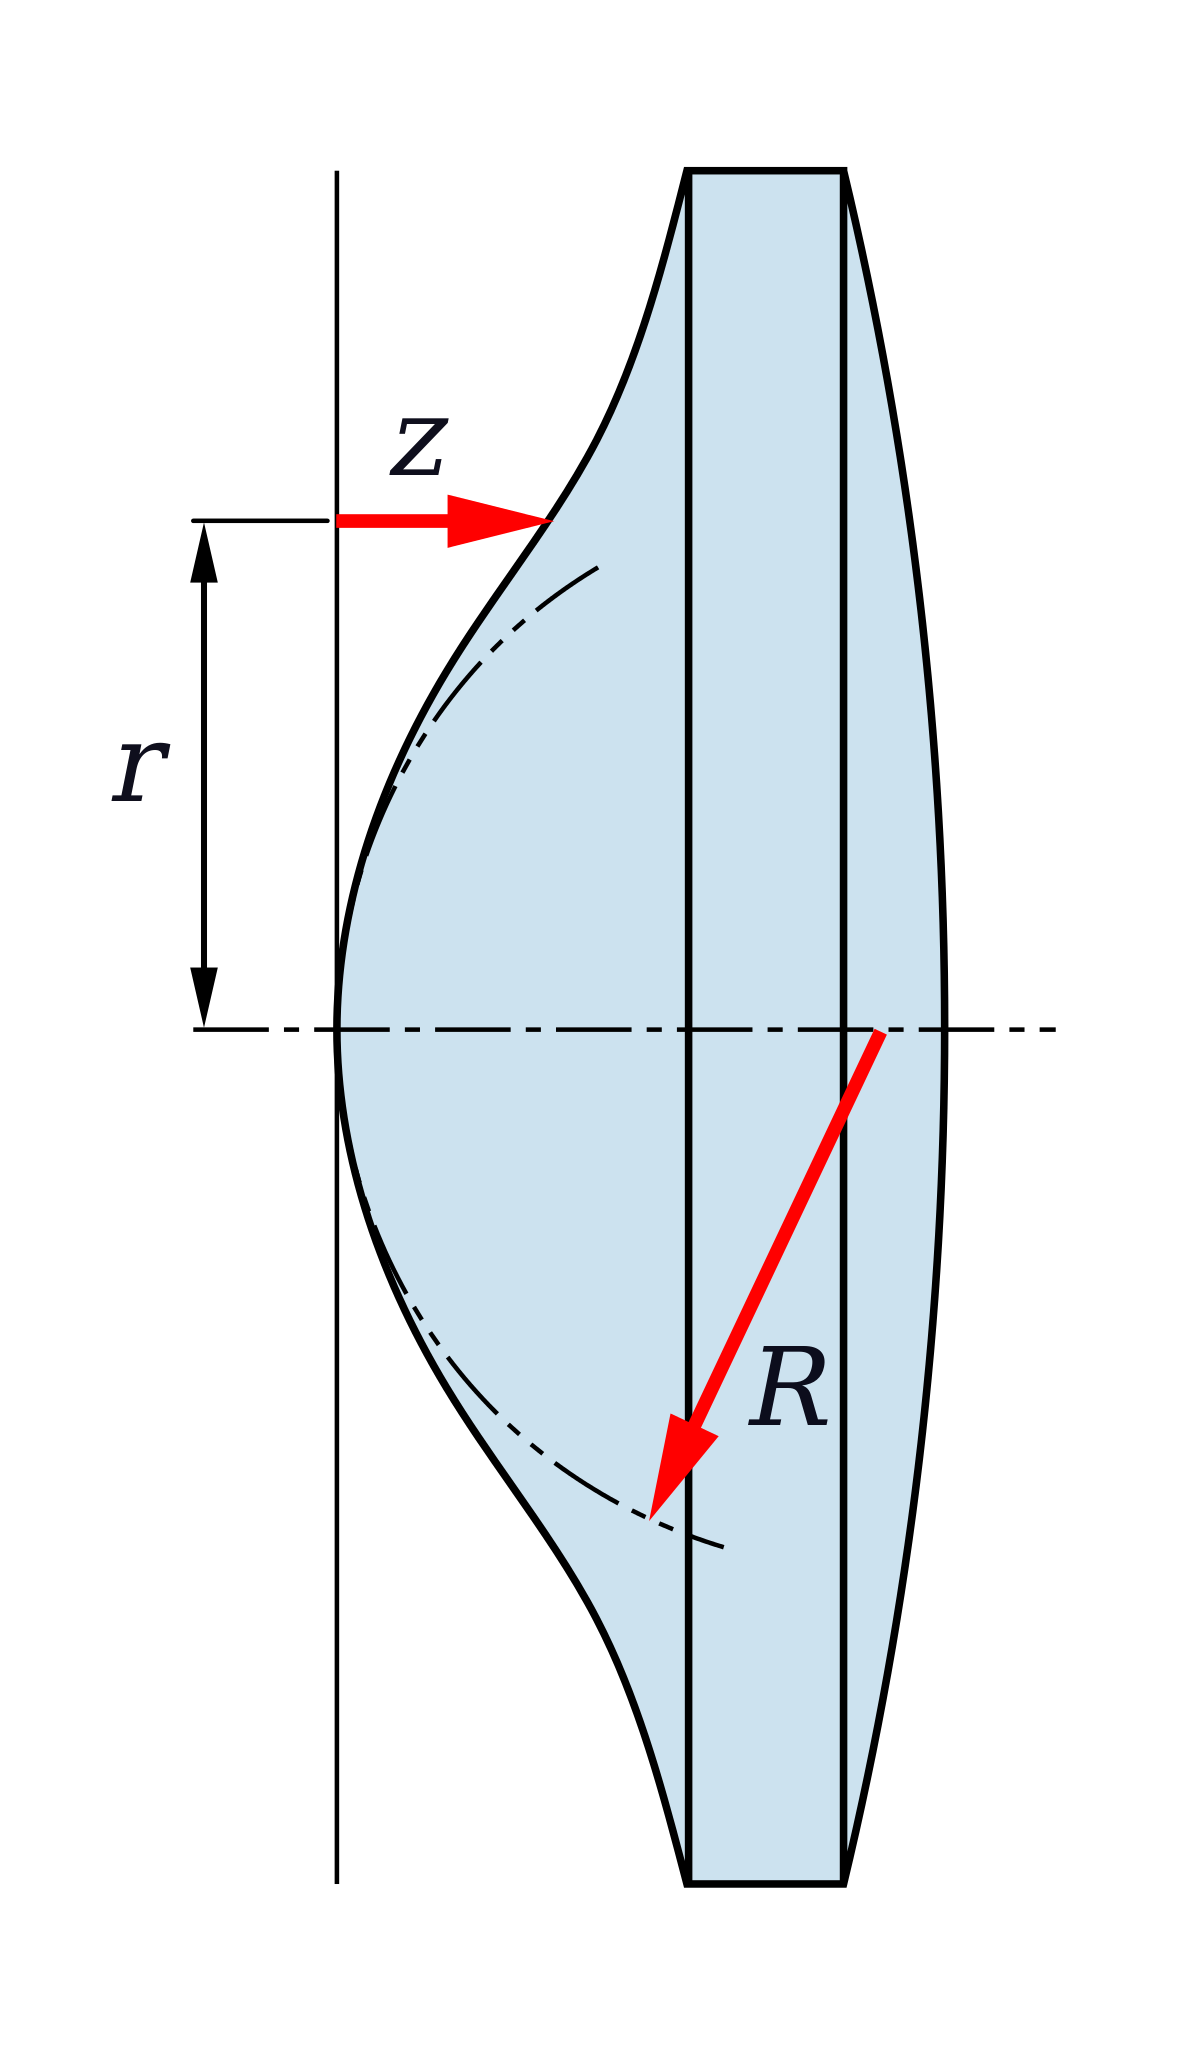
\includegraphics[width=3cm]{obrazky-figures/asphericLen.png}
\caption{Asférická šošvka, ktorej tvar potláča sférickú aberáciu. Prevzaté z }
\end{figure}

Týkala sa aj Hubblového teleskopu
\subsection{Coma}
Skreslenie off-axis objekov
\subsection{Petzvald field curvatore}
Riešenie: zakrivený senzor namiesto roviny.

\section{Chromatická aberácia}
Chromatická aberácia je jav šošovky, kedy jednotlivé vlnové dĺžky sú odlišne lomené pri dopade na
rozhranie šošovky. Dôsledkom toho je posunutie jednotlivých farebných zložiek v obraze, ktoré je
znázornené na obrázku \ref{chromaticAexample}.
Je spôsobená disperziou (rozptylom) svetla podľa vlnových dĺžok.

Obkec k obrazku = mozeme pozorovat, ze jednotlivé vlnové dlzky sú lomené pod iným uhlom, čo je
dosledok Snelloveho zakona.
\begin{figure}[h]
\centering
\label{chromaticAexample}
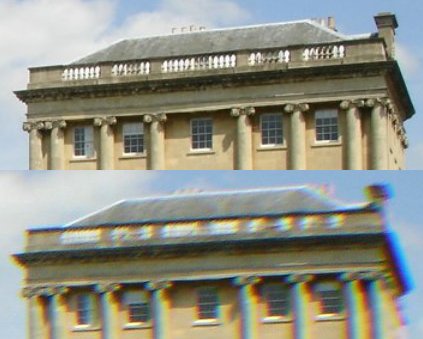
\includegraphics[width=6cm]{obrazky-figures/chromaticAberrationWikipedia.jpg}
\caption{lol}
\end{figure}

Riešenie: existujú SW \cite{automaticRemovalCA} ktoré sa pokúšajú o korekciu, 
existujú špeciálne šošovky, ktoré korektne lomia 2 vlnové dĺžky (doublet) alebo viacero
https://en.wikipedia.org/wiki/Achromatic\_lens

\section{Komplexné riešenia aberácii}
\begin{itemize}
    \item stop shifting = do optickej trasy sú umiestnené ďalšie uzávierky => blokovanie paprskov
        mimo optickej osy, ale vinetácia obrazu \cite{josesasian}
\end{itemize}
